\section{Deep learning}
Deep learning is a specialized branch of machine learning that focuses on training artificial neural networks with many layers.
These layers are the core building blocks that enable deep learning models to learn complex patterns and representations from vast amounts of data.
This approach has led to significant breakthroughs in various AI tasks, outperforming traditional machine learning methods in many applications \cite{lecunDeepLearning2015}.

\begin{figure}[hbtp]
    \centering    
    \begin{tikzpicture}[
    neuron/.style={circle,fill=blue!20,draw=black,minimum size=17pt,inner sep=0pt},
    input/.style={neuron, fill=green!20},
    output/.style={neuron, fill=red!20},
    hidden/.style={neuron, fill=blue!20},
    weight/.style={->,>=stealth'},
]

% Input layer
\foreach \name / \y in {1,...,4}
  \node[input] (I-\name) at (0,-\y) {};

% Hidden layer 1
\foreach \name / \y in {1,...,5}
  \node[hidden] (H1-\name) at (2.5,-\y+0.5) {};

% Hidden layer 2
\foreach \name / \y in {1,...,5}
  \node[hidden] (H2-\name) at (5,-\y+0.5) {};

% Output layer
\foreach \name / \y in {1,...,4}
  \node[output] (O-\name) at (7.5,-\y) {};

% Connect every node in the input layer with every node in the hidden layer 1
\foreach \source in {1,...,4}
  \foreach \dest in {1,...,5}
    \path[weight] (I-\source) edge (H1-\dest);

% Connect every node in the hidden layer 1 with every node in the hidden layer 2
\foreach \source in {1,...,5}
  \foreach \dest in {1,...,5}
    \path[weight] (H1-\source) edge (H2-\dest);

% Connect every node in the hidden layer 2 with every node in the output layer
\foreach \source in {1,...,5}
  \foreach \dest in {1,...,4}
    \path[weight] (H2-\source) edge (O-\dest);

% Annotate the layers
\node[above=0.5 of I-1] {Input layer};
\node[above=0.4 of H1-1, align=center] {Hidden\\layer 1};
\node[above=0.4 of H2-1, align=center] {Hidden\\layer 2};
\node[above=0.5 of O-1] {Output layer};

\end{tikzpicture}

    \caption{TODO: classic ANN diagram}
    \label{fig:ann}
\end{figure}

In the context of artificial neural networks, a layer is a collection of interconnected nodes, or neurons, that process information.
Each connection between two neurons has an associated weight (also known as a parameter), which is a numerical value that determines the strength of the connection.
These weights, play a crucial role in the learning process of a neural network.

\begin{figure}[hbtp]
    \centering    
    \begin{tikzpicture}[
    neuron/.style={circle,draw=black,minimum size=24pt,inner sep=0pt},
    input/.style={neuron, fill=blue!20},
    activation/.style={neuron, fill=yellow!20},
    sum/.style={neuron, fill=green!20},
    bias/.style={neuron, fill=red!20},
    arrow/.style={->,>=stealth'},
]
% input nodes
\node [input] (x1) at (0,1.5) {$x_1$};
\node [input] (x2) at (0,0) {$x_2$};
\node [input] (x3) at (0,-1.5) {$x_3$};
% sum node
\node [sum] (sum) at (2.5,0) {$\Sigma$};
% bias node
\node [bias] (bias) at (2.5,-1.5) {$b$};
% activation node
\node [activation] (activation) at (3.75,0) {$f$};
% output node
\node [] (y) at (5,0) {$y$};

% inputs to sum
\draw [arrow] (x1) -- node[above] {$w_{1}$} (sum);
\draw [arrow] (x2) -- node[above] {$w_{2}$} (sum);
\draw [arrow] (x3) -- node[above] {$w_{3}$} (sum);
% sum to activation
\draw [arrow] (sum) -- (activation);
% activation to output
\draw [arrow] (activation) -- node[right] {} (y);
% bias to sum
\draw [arrow] (bias) -- (sum);
\end{tikzpicture}

    \caption{Neuron} % TODO explain
    \label{TODO}
\end{figure}

Each layer performs a specific computation on the data it receives from the previous layer.
A neuron that receives input values from its connected neurons multiplies this value by their corresponding weights before being aggregated by the receiving neuron.
This aggregation is a simple summation, resulting in a weighted sum of the input values.
The neuron then applies a non-linear transformation to this weighted sum to produce its output.

A deep learning model typically consist of multiple layers stacked on top of each other, forming a hierarchical structure.
This structure allows the network to learn increasingly complex representations of the data as it flows through the layers.

Different types of layers serve different purposes in a deep learning model:
\begin{description}
    \item[Input layer:] 
    The first layer in the network, responsible for receiving the initial input data.
    Each neuron in this layer represent a feature of the input data, such as the pixel values in an image or the words in a sentence.
    \item[Hidden layer:] 
    Intermediate layers that lie between the input and output layers.
    They perform computations on the data received from the input, extracting features and learning increasingly abstract representations.
    Each hidden layer typically consists of many neurons, each applying a non-linear transformation (i.e., an activation function) to the weighted sum of its inputs.
    The activation function determines whether a neuron ``activates''.
    A neuron is said to be activated when its output is significant enough to contribute to the next layer's computations.
    \Cref{fig:activation_functions} shows activation functions that are commonly used: $\relu$, $\tanh$ and $\sigma$ (sigmoid).

    \begin{figure}[hbtp]
        \centering    
        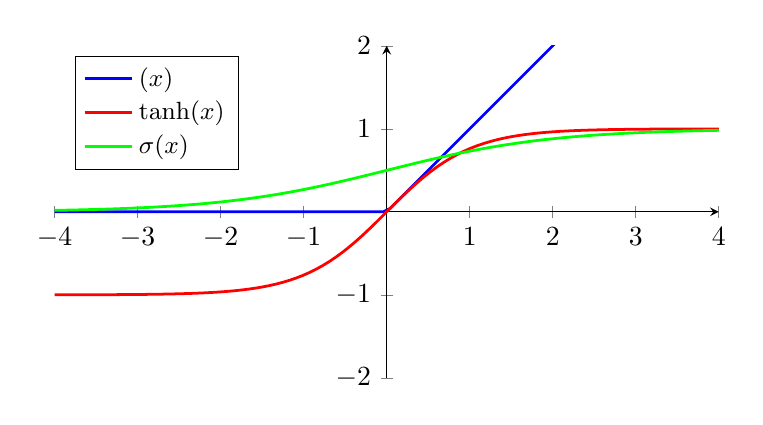
\begin{tikzpicture}
    \begin{axis}[
        axis lines = left,
        y=30,
        x=30,
        ymin = - 2, ymax = 2,
        xmin = -4, xmax = 4,
        axis lines=middle,
        legend pos={north west},
        legend cell align={left},
        legend style={font=\small},
    ]

    \addplot [
        domain=-4:4, 
        samples=100, 
        color=blue,
        line width=1pt
    ]
    {(x + abs(x)) / 2};
    \addlegendentry{$\relu(x)$}
    
    \addplot [
        domain=-4:4, 
        samples=100, 
        color=red,
        line width=1pt
    ]
    {tanh(x)};
    \addlegendentry{$\tanh(x)$}

    \addplot [
        domain=-4:4, 
        samples=100, 
        color=green,
        line width=1pt
    ]
    {e^x / (1 + e^x)};
    \addlegendentry{$\sigma(x)$}
    \end{axis}
\end{tikzpicture}

        \caption{Commonly used activation functions}
        \label{fig:activation_functions}
    \end{figure} 


    The number of hidden layers and neurons in each layer determines the depth and complexity of the network.
    \item[Output layer:] 
    The final layer, producing the result of the network's computation.
    The number of neurons in the output layer depends on the specific task, such as a classification label for image recognition or predicted value for natural language generation \cite{goodfellowDeepLearning2016}.
\end{description}

ANNs learn by adjusting the weights of the connections between neurons.
This process is called training and involves feeding the network with labeled data and iteratively updating the weights to minimize the difference between the network's predictions and the true labels.
The most common algorithm for training ANNs is backpropagation \cite{rumelhartLearningRepresentationsBackpropagating1986}, which calculates the gradient of the error with respect to each weight and updates the weights accordingly.

\subsection{Convolutional neural network}
Convolutional neural networks (CNNs) are a specialized class of artificial neuron networks designed to process data with inherent spatial structure, such as images.

A key element that sets them apart is the convolutional layer.
CNNs leverage the concept of convolution to extract local features.
The network then uses these extracted features to construct increasingly complex understandings of the input as the data progresses through its layers
\begin{figure}[hbtp]
    \centering    
    \begin{tikzpicture}[
    input/.style={matrix of nodes,
          nodes={draw, minimum size=5mm, fill=yellow!30},
          column sep=-\pgflinewidth, row sep=-\pgflinewidth,
          nodes in empty cells,
          },
    kernel/.style={matrix of nodes,
          nodes={draw, minimum size=5mm, fill=red!30},
          column sep=-\pgflinewidth, row sep=-\pgflinewidth,
          nodes in empty cells,
          },
    feature/.style={matrix of nodes,
          nodes={draw, minimum size=5mm, fill=green!30},
          column sep=-\pgflinewidth, row sep=-\pgflinewidth,
          nodes in empty cells,
          },
  ]
  
  % Input matrix
  \matrix[input] (mat1)
  {
  1 & 2 & 1 & 0\\
  0 & 1 & 1 & 1\\
  3 & 0 & 1 & 2\\
  1 & 1 & 0 & 1\\
  };
  \node[below=0.1cm of mat1] {Input};
  
  % Kernel matrix
  \matrix[kernel, above right=0.5cm and 1cm of mat1] (mat2)
  {
  0 & 1 & 0\\
  1 & 1 & 1\\
  0 & 1 & 0\\
  };
  \node[above=0.1cm of mat2] {Kernel};
  
  % Feature map matrix
  \matrix[feature, below right=0.5cm and 1cm of mat2] (mat3)
  {
  4 &  \\
   &  \\
  };
  \node[below=0.1cm of mat3] {Feature Map};
  
  % Draw lines
  \draw[blue!30, thin] (mat1-1-1.north west) -- (mat2-1-1.north west);
  \draw[blue!30, thin] (mat1-3-3.south east) -- (mat2-3-3.south east);
  
  % Highlight the receptive field
  \draw[red, thick, dashed] (mat1-1-1.north west) -- (mat1-1-3.north east) -- (mat1-3-3.south east) -- (mat1-3-1.south west) -- cycle;
  
\end{tikzpicture}

    \caption{
        This convolution operation involves a 3x3 kernel sliding across the input matrix.
        At each step, the kernel covers a receptive field (highlighted) and computes a weighted sum of the input values.
        This example shows one such step, resulting in the value 4 in the feature map.
    }
\end{figure}
A convolution operation involves sliding a learnable filter, or kernel, across the input data.
At each position, the filter performs an element-wise multiplication with the corresponding input data and sums the results.
This produces a single value in the output feature map.
By applying different filters, the network learns to detect various patterns like edges and shapes.

\begin{figure}[hbtp]
    \centering    
    \begin{tikzpicture}[
    input/.style={matrix of nodes,
          nodes={draw, minimum size=5mm, fill=green!30},
          column sep=-\pgflinewidth, row sep=-\pgflinewidth,
          nodes in empty cells,
          },
    pool/.style={matrix of nodes,
          nodes={draw, minimum size=5mm, fill=blue!30},
          column sep=-\pgflinewidth, row sep=-\pgflinewidth,
          nodes in empty cells,
          },
  ]
  
  % Input matrix (feature map)
  \matrix[input] (mat1)
  {
  1 & 2 & 2\\
  0 & 3 & 4\\
  5 & 1 & 2\\
  };
  \node[below=0.1cm of mat1] {Feature Map};
  
  % Pooling matrix (moved higher)
  \matrix[pool, above right=0cm and 1.5cm of mat1] (mat2)
  {
  3 & 4  \\
  5 & 4 \\
  };
  \node[below=0.2cm of mat2] {Pooled Feature Map};
  
  % Draw lines
  \draw[red!30, thin] (mat1-1-1.north west) -- (mat2-1-1.north west);
  \draw[red!30, thin] (mat1-2-2.south east) -- (mat2-1-1.south east);
  
  
  % Highlight the pooling window
  \draw[red, thick, dashed] (mat1-1-1.north west) -- (mat1-1-2.north east) -- (mat1-2-2.south east) -- (mat1-2-1.south west) -- cycle;
  
\end{tikzpicture}

    \caption{
        Max pooling operation with a 2x2 pooling window.
        In this example, the maximum value (3) within the highlighted region of the input feature map is extracted and placed in the pooled feature map.
    }
\end{figure}

The output of convolutional layers is then typically passed through pooling layers.
Pooling downsamples the feature map, reducing their dimensionality and making the network more robust to variations in the input.
Common pooling operations include taking the maximum or average value within a local region. % show pooling img

The use of activation functions introduces non-linearity, which enables the learning of complex patterns.
These activation functions are applied to the output of the convolutional and pooling layers.
% Common choices for such function are ReLU, sigmoid and tanh.

Finally, fully connected layers are often used in the final stages of a CNN.
These layers connect every neuron in the previous layer to every layer in the current layer.
This enables high-level reasoning and decision-making based on the extracted features.

The combining of simpler features into more complex ones across layers makes CNNs excel in computer vision tasks like image classification, object detection and image segmentation \cite{krizhevskyImageNetClassificationDeep2017}.

\subsection{Model optimizations}
Reducing the memory footprint of neural networks is an actively researched topic \cite{neillOverviewNeuralNetwork2020, leEfficientNeuralNetworks2023}.
Model compression involves refining a model to ensure it can function on devices with limited computational power, memory, and energy.
The goal is to maintain the model's performance while reducing resource demands.

Quantization focuses on reducing the numerical precision of a neural network's parameters.
Instead of relying on resource-intensive, high-precision floating-point numbers, quantization techniques employ lower-bit representations.
This reduction in precision translates to significant savings in memory and computational costs \autocite{guoSurveyMethodsTheories2018}.

Pruning techniques strategically remove less important components from a neural network.
This can involve eliminating individual weights, entire neurons, or even complete layers.
By simplifying the network architecture, pruning reduces its memory footprint and improves computational efficiency \cite{blalockWhatStateNeural2020}.
Different pruning strategies exist, including unstructured pruning, which removes individual weights based on their importance, and structured pruning, which eliminates entire filters within convolutional layers.

Beyond applying compression techniques to existing models, researchers are actively exploring novel neural network architectures that are inherently more efficient.
One such example is the residual neural network (ResNet) \autocite{heDeepResidualLearning2015}.
ResNets introduce skip connections, which allow the input of a layer to bypass one or more subsequent layers.
This seemingly simple modification has a major impact, enabling the training of much deeper networks while mitigating the vanishing gradient problem \cite{pascanuDifficultyTrainingRecurrent2012}.
Skip connections provide an alternate path for gradients to flow during backpropagation, preventing them from diminishing excessively as they travel through many layers.
This allows ResNets to learn more complex features and achieve higher accuracy with fewer parameters. 

\begin{figure}[hbtp]
\centering    
\includegraphics[width=3cm]{example-image-a}
\caption{TODO: ResNet image}
\end{figure}